\chapter[Software]{Software}
    \section{Arquitetura de software}

	\begin{flushright}
		\begin{minipage}[c]{.65\textwidth}
		
		
		{\small “Gather together those things that change for the same reason, and separate those things that change for different reasons.” - Single Responsibility Principle - Robert C. Martin}
		
		
		\end{minipage}
	\end{flushright}

    A Arquitetura proposta para este trabalho é baseada nos princípios de Micro Serviços. Estes são uma solução em forma de componentes de software menores e autônomos focados em tarefas específicas, para promover o reuso de software e bases de código de maior manutenibilidade e coesão com baixo acoplamento \cite{newman_2018}.

    Um problema comum em softwares monolíticos é o rastreamento de mudanças e a definição de fronteiras entre funções similares que geram código repetido espalhados pela aplicação, e podem dificultar a correção de bugs ou tornar implementações mais complexas \cite{newman_2018}. Esse impacto na manutenibilidade do software e evolução do RICC é um ponto crítico na decisão desta arquitetura de acordo com os princípios da Gerência de Configuração e Evolução de Software \cite{gces} e o Princípio da Responsabilidade Única de Robert C. Martins.

    Os Micro Serviços utilizam estes princípios de código para criação serviços independentes. Focando as divisões de um serviço em fronteiras de negócio. Então se torna óbvio onde um determinado código estará para uma funcionalidade específica. Mantendo um serviço dentro de suas responsabilidades escapamos das tentações de aumentar a complexidade do módulo e todas as dificuldades associadas com esta decisão \cite{newman_2018}.

    \begin{figure}[H]
        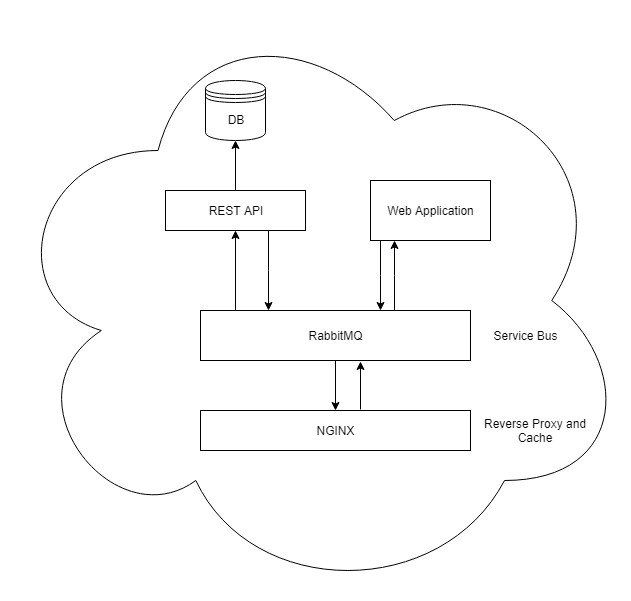
\includegraphics[width=\textwidth]{software/images/arquitetura.png}
        \caption{Arquitetura do servidor.}
        \label{fig:arquitetura}
    \end{figure}

    A arquitetura \ref{fig:arquitetura} aqui proposta, busca amplificar os seguintes benefícios para o projeto: Heterogeneidade de tecnologias; Resiliência do sistema; Escalabilidade; Facilidade de Implantação e Atualizações; Composição de serviços; e Otimização para Substituições.

    A Heterogeneidade de Tecnologias é um ponto chave do trabalho, pois permite que a equipe utilize as ferramentas ideais para cada trabalho, otimizando pontos fortes de uma tecnologia sem a necessidade de estender suas atividades além de seu principal domínio. Onde por exemplo escolhemos o Framework Django REST para nossa API de dados e o Django para o servidor principal \ref{fig:arquitetura}, não necessitando a fusão das tecnologias para cumprir um papel monolítico.

    A Resiliência de um sistema está relacionada a falhas e problemas. Onde uma determinada falha não é capaz de criar uma cascata de falhas derrubando todo o sistema, assim, podemos isolar um problema e manter os outros serviços funcionando normalmente. Então, caso tenhamos uma falha no servidor de aplicação e processamento de informações, a API de dados continua disponível e isolada do problema para seus usuários.
    
    Para nossa aplicação com grande armazenamento de dados dos sensores de estações e o processamento dos mesmos, a Escalabilidade monolítica não é uma opção, pois seria necessário escalar todos serviços juntos. Esta decisão de arquitetura permite evoluções nos módulos de armazenamento e processamento, sem necessariamente impactar nos outros serviços, economizando recursos dos servidores e financeiros para o projeto em casos de ajuste e escala.
    
    Estas separações entre aplicações também buscam facilitar a Implantação e atualização destes serviços de forma independente. A infraestrutura disponível na FGA é instável e a mobilidade do sistema para outras nuvens e máquinas é ponto chave para a alta disponibilidade do software. Em casos de atualizações pontuais a serviços, não se torna obrigatório a atualização de todos os sistemas rodando, apenas dos impactados pelas correções.
    
    Por último, temos as capacidades de Composição e a Otimização para Substituições. A utilização destes módulos separados que formam nosso sistema, permite e facilita o reuso destes serviços em outros contextos, e é característica fundamental para a equipe. Onde também é possível realizar substituições de uma ferramenta por outra que atenda a funcionalidade e o protocolo definido pelo serviço em substituição.

    \subsection{Protocolos de comunicação}
    
    Segundo a RFC que o define, \cite{rfc}, o Protocolo de Transferência de Hipertexto (HTTP) é um protocolo a nível de aplicação para informações distribuídas, colaborativas e de hipermídia entre sistemas. Possui diversas tarefas além de seu uso com Hipertexto, através da extensão de seus métodos de requisição, códigos de erro e cabeçalhos. É também utilizado como um protocolo genérico de comunicação entre agentes e proxies para outros sistemas de internet. 

    O HTTP é um protocolo de Requisição e Respostas, onde um cliente envia uma requisição a um servidor na forma de um método de requisição, URI e versão do protocolo, seguido de uma mensagem contendo modificadores da requisição, informações do cliente e possivelmente um conteúdo em relação a conexão com o servidor. O Servidor responde com uma linha de status, incluindo o versão do protocolo da mensagem e um código de sucesso ou erro, seguido de uma mensagem contendo informações do servidor, entidade e possivelmente um conteúdo \cite{rfc}.

    Como na maioria das conexões seguindo HTTP ela será iniciada pelo usuário buscando uma requisição que seja aplicada em um recurso do servidor. Em nosso contexto, o usuário criando a requisição serão os módulos centrais que estarão enviando dados dos sensores a serem salvos na API de armazenamento e esta comunicação será autenticada via tokens criptográficos nos cabeçalhos das requisições.

    \begin{figure}[H]
        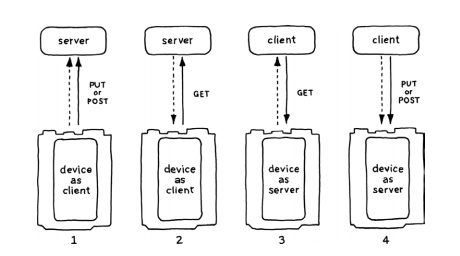
\includegraphics[width=\textwidth]{software/images/figura_http.png}
        \caption{Figura 4-5 retirada do livro \cite{pfister_2011}}
        \label{fig:http}
    \end{figure}

    As centrais utilizarão os requisições HTTP com os métodos POST para o envio de dados da sua rede para armazenamento remoto em nuvem e GET para a obtenção de recursos e polling periódico de atualizações com o servidor. \cite{pfister_2011}. Estaremos então seguindo os padrões 1 e 2 da figura \ref{fig:http}, pois não é viável que todas os módulos centrais possuam um endereço de IP público que seja acessível pelo servidor da aplicação para iniciar a comunicação.
    
    Segundo \cite{ohara_2007}, o Advanced Message Queuing Protocol (AMQP) é um padrão aberto de camada de aplicação para middlewares orientados a mensagens. Os pontos principais deste protocolo são message orientation, queuing, routing, reliability e security .
    Este protocolo permite que diferentes implementações de sistemas consigam se comunicar entre si, criando uma interoperabilidade de sistemas e consequentemente facilitando a escalabilidade de todo um ecossistema de software.
    Este protocolo classifica os sistemas em publishers e consumers, onde os primeiros publicam mensagens para os brokers (roteadores de mensagens), que em seguida são destinadas aos consumers.
    O broker de mensagens que utilizaremos será o RabbitMQ, uma tecnologia aberta, amplamente utilizada e testada para este tipo de protocolo.
    
    \begin{figure}[H]
        \centering
        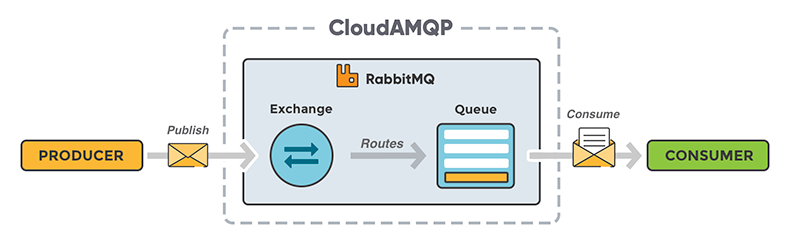
\includegraphics[width=\textwidth]{software/images/amqp.png}
        \caption{Protocolo AMQP}
        \label{fig:amqp}
    \end{figure}

    \section{Modelagem das aplicações}
    
    Nossa solução consiste em basicamente 5 módulos, divididos seguindo  o Princípio da Responsabilidade Única de Robert C. Martins. Cada um destes módulos executará em diferentes dispositivos, para formar o  ecossistema RICC. São eles:
    
    \subsection{Aplicação Web}

    Aplicação que irá executar dentro de um navegador, possuindo todas as funcionalidades disponíveis para os usuários (visualizar dados, controlar a irrigação).
	Esta aplicação irá interagir com a API de consulta, tanto para receber os dados exibidos, quanto para enviar comandos para os sistemas de irrigação.

    \begin{figure}[H]
    	
    	\centering
        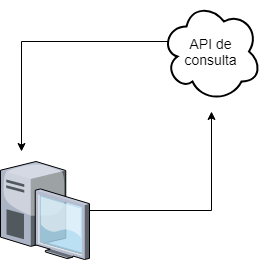
\includegraphics[width=.5\textwidth]{software/images/web.png}
        \caption{Aplicação web}
        \label{fig:web}
    \end{figure}

    \subsection{Aplicativo mobile}

    Esta aplicação possuirá as mesmas funcionalidades da aplicação web, porém executará em dispositivos móveis, usufruindo de funcionalidades nativas de cada plataforma, como o sistema de notificações.

    \begin{figure}[H]
    	
    	\centering
        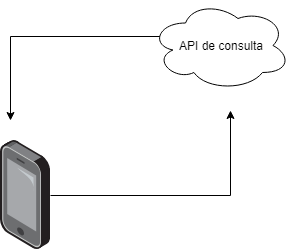
\includegraphics[width=.5\textwidth]{software/images/mobile.png}
        \caption{Aplicativo mobile}
        \label{fig:mobile}
    \end{figure}

    \subsection{API de dados}

    Este sistema ficará disponível em um servidor web, que terá a função de guardar dados de sensores genéricos, sendo facilmente extensível para novos tipos de dados. Possuindo esta única responsabilidade, melhorando a escalabilidade horizontal deste serviço.

    \subsection{API de consulta}

    A API de consulta servirá como uma interface entre as aplicações utilizadas pelos usuários (Aplicação Web e Aplicação Mobile), além de ter o módulo de autenticação e criação de novos usuários.

    \begin{figure}[H]
    	\centering
        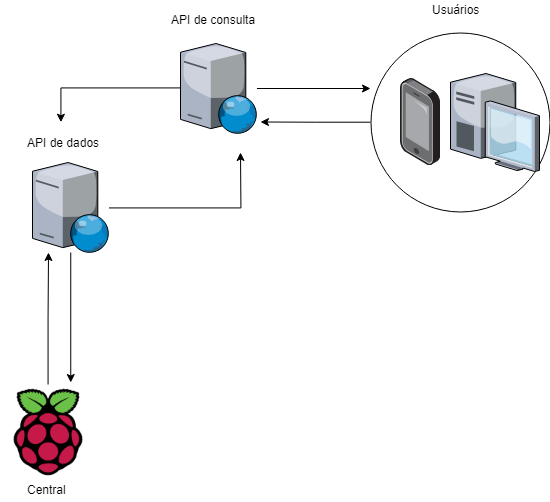
\includegraphics[width=.8\textwidth]{software/images/apidados.png}
        \caption{Esquemático das API's}
        \label{fig:apidados}
    \end{figure}

    \subsection{Central}

    O sistema central possuirá um sistema híbrido de linguagens, que servirá de gateway  tanto para a os dados decorrentes da rede mesh serem transmitidos pela internet, quanto para transmitir as interações do usuário sobre os sistemas de irrigação, para a rede mesh. 
	De acordo com a modelagem deste projeto, teremos diversas estações centrais espalhadas por diferentes redes de internet, tornando inviável um endereçamento de IP público para cada estação, assim, este tipo de endereçamento público será feito apenas para os servidores.
    
    Para que seja então possível receber informações periódicas do servidor em cada estação Central, será implementado um sistema de Polling/WebSocket com requisições de GET de acordo com o protocolo HTTP. De acordo com pesquisas do Chromium \cite{chromium}, este tipo de requisição possuem cabeçalhos que pesam entre 200 bytes e 2KB, assim, em média com um sistema de polling a cada minuto, teríamos um gasto aproximado de banda de 45MB mensais.
    
    \begin{figure}[H]
    	\centering
        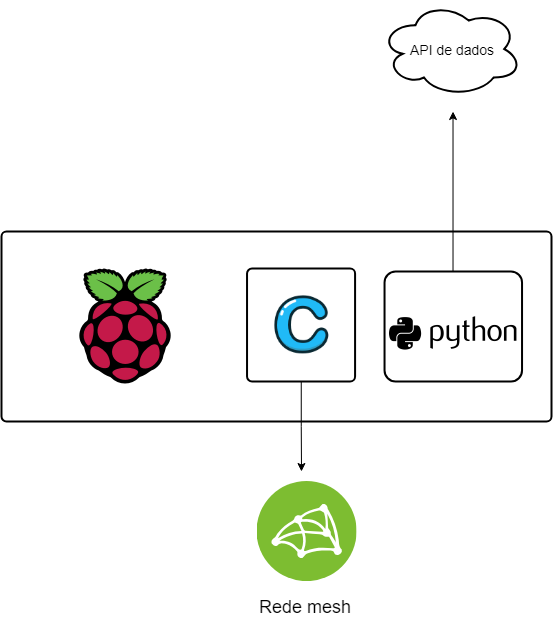
\includegraphics[width=.7\textwidth]{software/images/central.png}
        \caption{Diagrama do sistema da central.}
        \label{fig:central}
    \end{figure}

    \section{Casos de Uso}
    
    Os casos de uso descrevem em linguagem de alto nível as funcionalidades requeridas de cada sistema.

	\begin{table}[H]
		\centering		
		\caption{Atores}
        \label{tab:Atores}
		\begin{tabular}{|c|c|}
			\hline
				Ator     & Descrição                                                                                                                                                                                          			\\ \hline
				Usuário  & \begin{tabular}[c]{@{}c@{}}Usuário que utilizará o nosso sistema através \\ do 					aplicativo mobile ou aplicação web.\end{tabular}                                                                    			\\ \hline
			Estação  & \begin{tabular}[c]{@{}c@{}}Sistema responsável por coletar os dados fornecidos \\ 				pelos sensores e enviar estes dados na rede mesh, \\ para que fiquem disponíveis no módulo 					central.\end{tabular} \\ \hline
			Atuador  & \begin{tabular}[c]{@{}c@{}}Sistema responsável por ligar o sistema de irrigação \\ 				e comunicar o estado (ligado/desligado) do mesmo.\end{tabular}                                                  			\\ \hline
			Central  & \begin{tabular}[c]{@{}c@{}}Sistema com acesso à internet, que será responsável por 				\\ enviar os dados de todas as estações, relacionadas a esta\\ central, para um servidor na 				nuvem.\end{tabular} \\ \hline
			Servidor & \begin{tabular}[c]{@{}c@{}}Microsserviços responsáveis por processar \\ os dados 				coletados de estações e disponibilizar \\ os resultados deste processamento, para os usuários.				\end{tabular}       \\ \hline
			Apps     & \begin{tabular}[c]{@{}c@{}}Aplicativos mobile e web que exibirá os dados, \\ 					coletados e processados, para os usuários.\end{tabular}                                                               			\\ \hline
		\end{tabular}
	\end{table}



		\begin{table}[H]
			\caption{Casos de uso}
	        \label{tab:usecase}
			\begin{tabular}{|c|c|l|}
				\hline
					\#   & Ator     & Nome                                                    \\ \hline
					UC01 & Estação  & Conectar a rede Mesh RF                                 \\ \hline
					UC02 & Estação  & Coletar dados dos sensores                              \\ \hline
					UC03 & Estação  & Armazenar dados coletados dos sensores                  \\ \hline
					UC04 & Estação  & Enviar dados para a Central                             \\ \hline
					UC05 & Estação  & Ativar Atuador                                          \\ \hline
					UC06 & Estação  & Notificar falha de sensores                             \\ \hline
					UC07 & Atuador  & Conectar a rede Mesh RF                                 \\ \hline
					UC08 & Atuador  & Ativar bomba de irrigação                               \\ \hline
					UC09 & Atuador  & Desativar bomba de irrigação                            \\ \hline
					UC10 & Atuador  & Informar estatus                                        \\ \hline
					UC11 & Central  & Conectar a rede Mesh RF                                 \\ \hline
					UC12 & Central  & Conectar a rede Ethernet                                \\ \hline
					UC13 & Central  & Receber dados enviados pelos nós da rede Mesh RF        \\ \hline
					UC14 & Central  & Armazenar dados enviados pelos nós da rede Mesh Rf      \\ \hline
					UC15 & Central  & Enviar dados da rede Mesh RF para o servidor            \\ \hline
					UC16 & Central  & Armazenar informações de configuração do usuário        \\ \hline
					UC17 & Central  & Receber dados enviados pelo servidor                    \\ \hline
					UC18 & Central  & Enviar dados recebidos do servidor para a rede Mesh RF  \\ \hline
					UC19 & Central  & Ativar atuador conectado a rede Mesh RF                 \\ \hline
					UC20 & Central  & Detectar falha de conexão em algum nó da rede Mesh RF   \\ \hline
					UC21 & Central  & Repassar falhas diagnosticadas nos nós, para o servidor \\ \hline
					UC22 & Servidor & Cadastrar novos usuários                                \\ \hline
					UC23 & Servidor & Logar novos usuários                                    \\ \hline
					UC24 & Servidor & Receber dados das centrais                              \\ \hline
					UC25 & Servidor & Armazenar dados das centrais                            \\ \hline
					UC26 & Servidor & Criar notificações para usuários                        \\ \hline
					UC27 & Usuário  & Efetuar cadastro                                        \\ \hline
					UC28 & Usuário  & Efetuar login                                           \\ \hline
					UC29 & Usuário  & Solicitar mudança de estado no atuador de irrigação     \\ \hline
					UC30 & Usuário  & Receber notificações sobre a plantação                  \\ \hline
					UC31 & Usuário  & Configurar sistema de notificações                      \\ \hline
					UC32 & Usuário  & Visualizar informações da Central                       \\ \hline
					UC33 & Usuário  & Visualizar informações de cada Estação                  \\ \hline
					UC34 & Usuário  & Visualizar informações de um atuador                    \\ \hline
			\end{tabular}
		\end{table}


    \section{Diagramas}

    \subsection{Diagramas de caso de uso}

    \begin{figure}[H]
    	\centering
        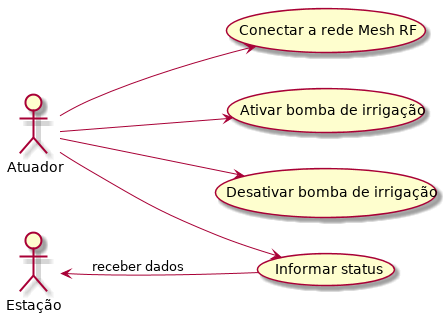
\includegraphics[width=.9\textwidth]{software/diagramas/casosDeUso/atuador.png}
        \caption{Diagrama de casos de uso de atuadores.}
        \label{fig:atuador}
    \end{figure}
    
    \begin{figure}[H]
        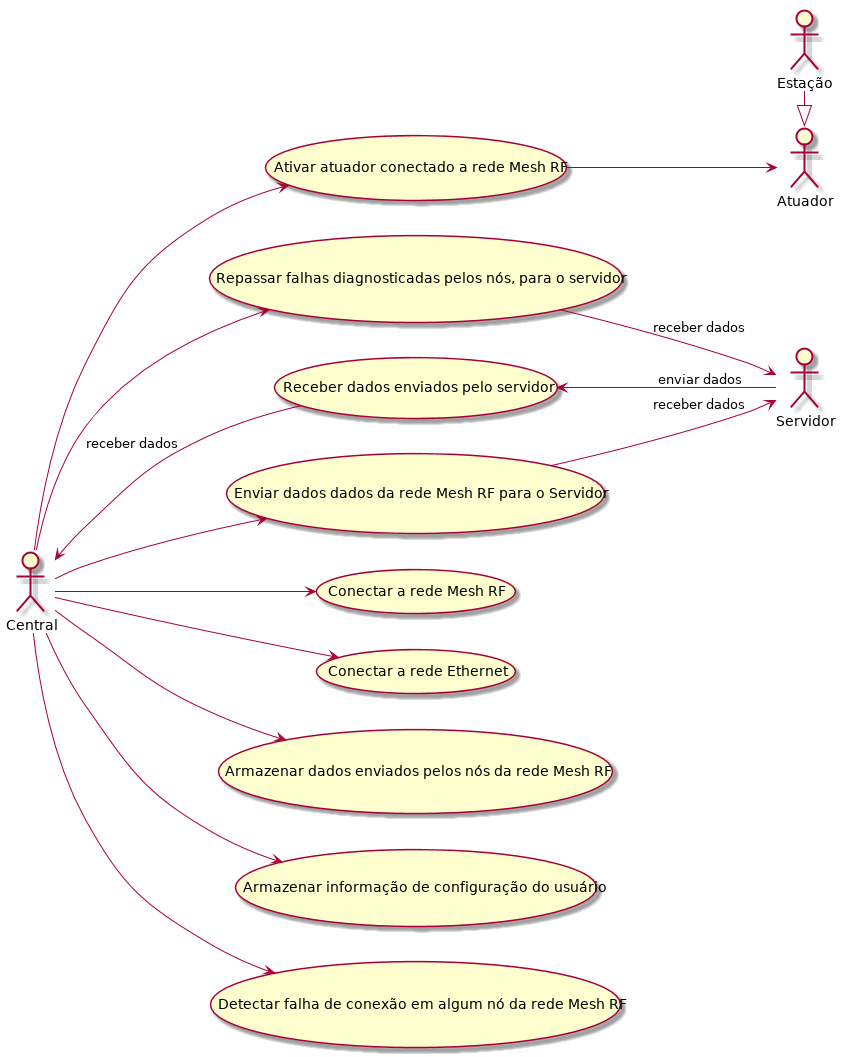
\includegraphics[width=\textwidth]{software/diagramas/casosDeUso/central.png}
        \caption{Diagrama de casos de uso de centrais.}
        \label{fig:central}
    \end{figure}

    \begin{figure}[H]
        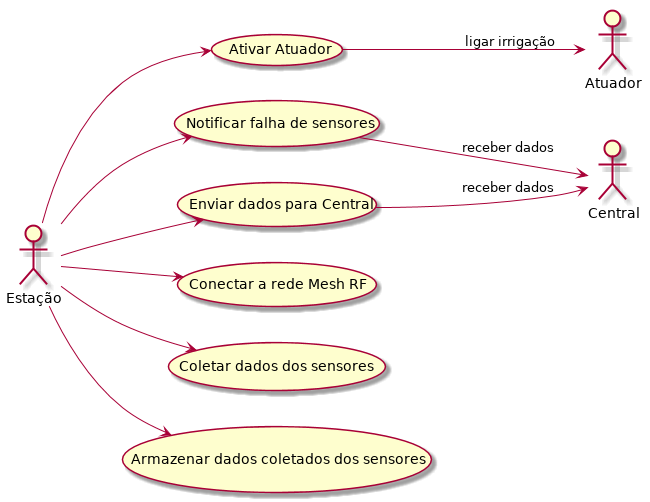
\includegraphics[width=\textwidth]{software/diagramas/casosDeUso/estacao.png}
        \caption{Diagrama de casos de uso de estações.}
        \label{fig:estacao}
    \end{figure}

    \begin{figure}[H]
    	\centering
        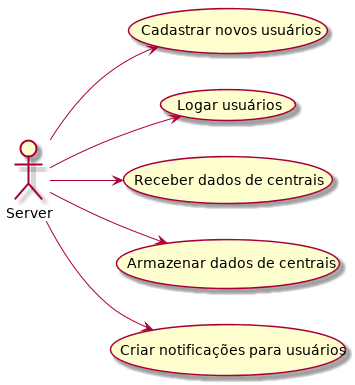
\includegraphics[width=.7\textwidth]{software/diagramas/casosDeUso/server.png}
        \caption{Diagrama de casos de uso de servidor.}
        \label{fig:server}
    \end{figure}

    \begin{figure}[H]
        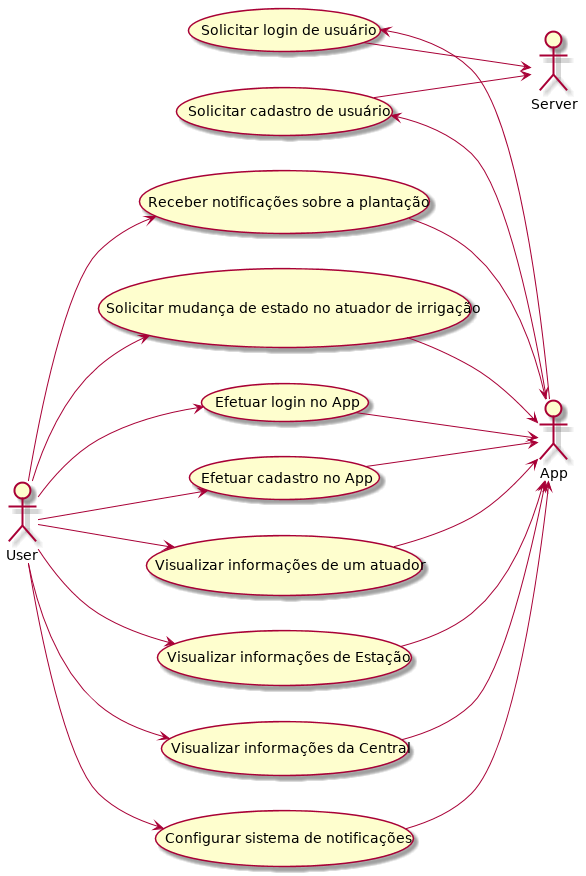
\includegraphics[width=\textwidth]{software/diagramas/casosDeUso/user.png}
        \caption{Diagrama de casos de uso de usuários.}
        \label{fig:user}
    \end{figure}
    

    \subsection{Diagrama de classe}
        
    \begin{figure}[H]
        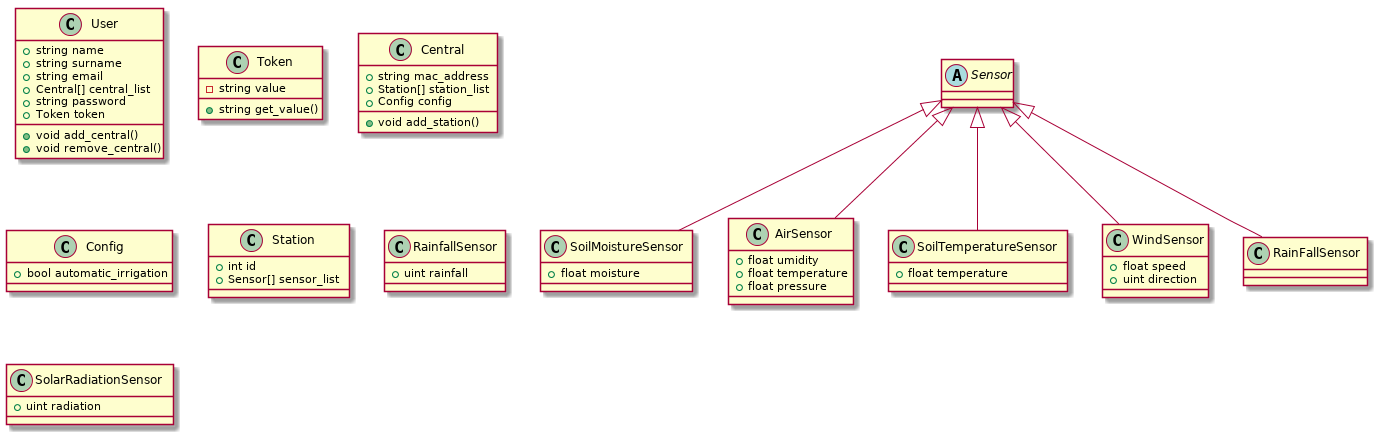
\includegraphics[width=\textwidth]{software/diagramas/classes/classes_server.png}
        \caption{Diagrama de classes do servidor.}
        \label{fig:classes}
    \end{figure}


    \subsection{Diagramas de sequência}

    \begin{figure}[H]
    	\centering
        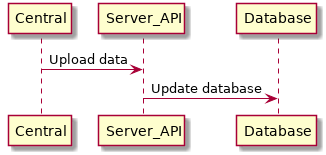
\includegraphics[width=.7\textwidth]{software/diagramas/sequencia/server.png}
        \caption{Diagrama de sequência do servidor.}
        \label{fig:sequence_server}
    \end{figure}

    \begin{figure}[H]
        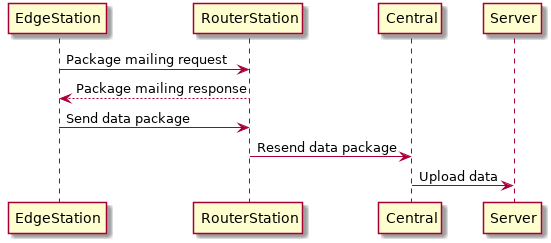
\includegraphics[width=\textwidth]{software/diagramas/sequencia/station.png}
        \caption{Diagrama de sequência da estação.}
        \label{fig:sequence_station}
    \end{figure}

	\section{Tecnologias}
	\subsection{Docker}
	Docker é uma plataforma para desenvolvimento, empacotamento e execução de aplicações. Permite que separemos a aplicação da infraestrutura para que possamos entregar o \textit{software} mais rapidamente. Utilizando esta tecnologia podemos gerenciar a infraestrutura dos microserviços da mesma forma que a aplicação, através de código. Este empacotamento também amplia muito a velocidade de atualização do ambiente de produção da nossa plataforma.
	
	Com Docker podemos empacotar e executar a aplicação em um ambiente isolado de contêiner. Esse isolamento permite que rodemos múltiplos contêineres simultaneamente em uma mesma máquina hospedeira, simulando um ambiente distribuído para os microserviços da nossa aplicação.
	Docker será responsável por:
	\begin{enumerate}
		\item Ambiente de desenvolvimento
		\item Isolamento de Serviços
		\item Unidade básica para distribuição da aplicação 
		\item Implantação da produção em nuvem publica.
	\end{enumerate}

	\subsection{Django REST}
		Django é um \textit{framework} para a linguagem Python na Web, que é conhecido por um desenvolvimento rápido e pragmático. É \textit{Open-Source} e possui uma comunidade ativa. Seus principais pontos fortes são: a velocidade; segurança; e escalabilidade.
		
		Acoplado ao Django utilizaremos o \textit{kit} REST para o desenvolvimento das Web APIs. Esta ferramenta trás algumas funcionalidades importantes para o projeto e velocidade do desenvolvimento, como: API navegável pelo navegador, permitindo validações e testes visuais; Políticas de autenticação com \textit{OAuth1} e \textit{OAuth2}; Serialização que suporta bancos de dados relacionais e não-relacionais, algo que permite melhor composição com outros serviços; Customizável e escalável caso precisemos de novas funcionalidades não previstas; Documentação e suporte da comunidade de desenvolvedores.

	\subsection{Angular}

	\subsection{NativeScript}

	\subsection{Python}

    \subsection{C Embarcado}
    A linguagem de programação que utilizaremos no desenvolvimentno do software que rodará
    nas estações, será a linguagem C embarcada. Esta variante da linguagem C é bastante otimizada
    para microcontroladores com recursos limitados de RAM, ROM e necessidade de controle de periféricos.
    Nós utilizaremos o compilador Gnu Compiler Collection (GCC), pois esta implementação possui várias flags
    de otimização para sistemas embarcados, possuir suportae a vários tipos de microcontroladores, possuir
    um sistema de debug (GDB) bastante eficiente, além de ser possível a chamada de código Assembly diretamente
    dentro do programa.